\chapter{Chemische reacties: beginstoffen en reactieproducten}\label{ch:g7:chemical-reactions}

Houtskool gloeit in een barbecue. Een uur later is er van de zwarte
brokken bijna niets meer over --- een beetje grijze as, en de warmte
waarmee het eten gaar werd. Waar is de zwarte koolstof gebleven? Hij is
niet verdwenen: hij heeft de zuurstof van de \omterm{def:g4:air-a-mixture-of-gases:air}{lucht} ontmoet en is een
nieuw, onzichtbaar gas geworden. Nu we \omterm{def:g7:atoms-and-molecules:atom}{atomen} en \omterm{def:g7:atoms-and-molecules:molecule}{moleculen} kennen, kunnen
we precies zeggen wat er bij zo'n verandering gebeurt.

\begin{recall}
Bij een \omterm{def:g5:irreversible-changes:chemical-change}{chemische verandering} ontstaan nieuwe stoffen en is er geen
eenvoudige weg terug (\cref{ch:g5:irreversible-changes}). Kalkwater wordt
troebel met koolstofdioxide, watervrij kopersulfaat wordt blauw met water
(\cref{ch:g7:identifying-substances}). Alle materie bestaat uit \omterm{def:g7:atoms-and-molecules:atom}{atomen},
die zich tot \omterm{def:g7:atoms-and-molecules:molecule}{moleculen} groeperen; een formule zoals \ce{CO2} somt de
\omterm{def:g7:atoms-and-molecules:atom}{atomen} van een \omterm{def:g7:atoms-and-molecules:molecule}{molecuul} op (\cref{ch:g7:atoms-and-molecules}).
\end{recall}

\begin{omfigure}
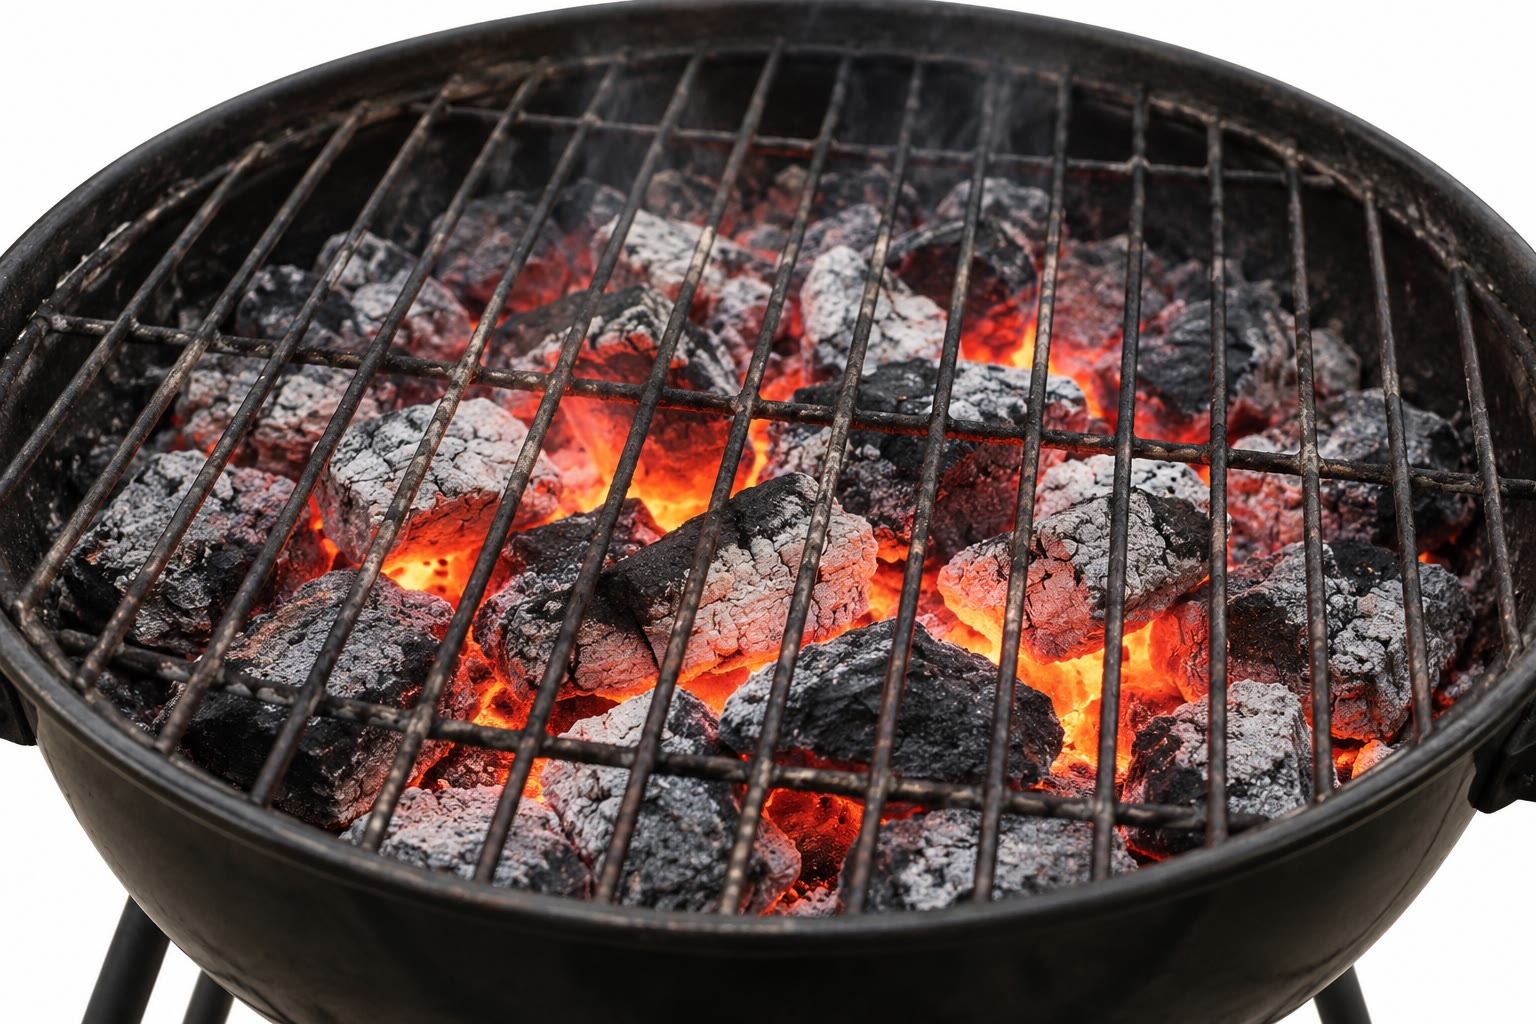
\includegraphics[width=0.55\linewidth]{images/book1/ai/g7-charcoal-bbq.jpg}

{\small Gloeiende houtskool: koolstof die reageert met de zuurstof van de
\omterm{def:g4:air-a-mixture-of-gases:air}{lucht}.}
\end{omfigure}

\section{Fysische en chemische veranderingen}

\begin{definition}[Fysische verandering]\label{def:g7:chemical-reactions:physical-transformation}
Een \emph{fysische verandering}\index{fysische verandering} verandert de
toestand of de ordening van materie zonder de \omterm{def:g6:pure-substances-and-mixtures:species}{chemische stoffen} te
veranderen: smelten, bevriezen, koken, \omterm{def:g2:mixing-and-dissolving:dissolve}{oplossen}, \omterm{def:g2:mixing-and-dissolving:mix}{mengen}. Voor en na zijn
dezelfde stoffen aanwezig; alleen hun vorm of hun ordening is veranderd.
\end{definition}

\begin{example}[Water, op drie manieren]\label{ex:g7:chemical-reactions:water}
IJs dat smelt tot water, water dat kookt tot waterdamp, en zout dat in
water \omterm{def:g2:mixing-and-dissolving:dissolve}{oplost}, zijn \omterm{def:g7:chemical-reactions:physical-transformation}{fysische veranderingen}: voor en na zijn er
watermoleculen (en zout). Als je inzoomt, zijn de \omterm{def:g7:atoms-and-molecules:molecule}{moleculen} dezelfde;
alleen hoe ze geordend zijn en hoe ze bewegen, is veranderd.
\end{example}

\begin{proposition}[Chemische omzetting]\label{prop:g7:chemical-reactions:chemical}
Bij een \omterm{def:g5:irreversible-changes:chemical-change}{chemische verandering}, ook wel chemische omzetting genoemd,
verdwijnen sommige \omterm{def:g6:pure-substances-and-mixtures:species}{chemische stoffen} en ontstaan er nieuwe. Je
onderscheidt haar van een \omterm{def:g7:chemical-reactions:physical-transformation}{fysische verandering} aan haar producten:
nieuwe stoffen, die je met \omterm{def:g7:identifying-substances:characteristic-test}{aantoningsreacties} kunt aantonen.
\end{proposition}

\begin{omfigure}
\begin{tikzpicture}[font=\small, level distance=1.5cm,
    box/.style={draw=omDef, fill=omDef!6, rounded corners=2pt, align=center,
      inner sep=4pt},
    level 1/.style={sibling distance=6.6cm},
    edge from parent/.style={draw, thick, omDef, ->}]
  \node[box] {een verandering van materie}
    child {node[box, text width=5.2cm] {\textbf{fysisch}: dezelfde stoffen\\
      voor en na\\ \footnotesize smelten, koken, oplossen, mengen}}
    child {node[box, draw=omProp, fill=omProp!6, text width=5.2cm]
      {\textbf{chemisch}: stoffen verdwijnen,\\ nieuwe stoffen ontstaan\\
      \footnotesize verbranden, roesten, koken van eten}};
\end{tikzpicture}

{\small Twee soorten veranderingen.}
\end{omfigure}

\section{Beginstoffen en reactieproducten}

\begin{definition}[Chemische reactie]\label{def:g7:chemical-reactions:reaction}
Een \emph{chemische reactie}\index{chemische reactie} is het model dat
scheikundigen gebruiken voor een chemische omzetting: het noemt de
stoffen die verbruikt worden en de stoffen die gevormd worden.
\end{definition}

\begin{definition}[Beginstoffen en reactieproducten]\label{def:g7:chemical-reactions:reactant}
De stoffen die bij een \omterm{def:g7:chemical-reactions:reaction}{chemische reactie} verbruikt worden, zijn de
\emph{beginstoffen}\index{beginstof}; de stoffen die gevormd worden, zijn
de \emph{reactieproducten}\index{reactieproduct}.
\end{definition}

\begin{example}[Koolstof die in zuurstof verbrandt]\label{ex:g7:chemical-reactions:carbon}
Als houtskool verbrandt, zijn de \omterm{def:g7:chemical-reactions:reactant}{beginstoffen} koolstof (de houtskool) en
zuurstof (uit de \omterm{def:g4:air-a-mixture-of-gases:air}{lucht}). Het \omterm{def:g7:chemical-reactions:reactant}{reactieproduct} is koolstofdioxide: als je
het gas dat in de pot achterblijft met kalkwater schudt, wordt dat
troebel.
\end{example}

\begin{inthelab}[Houtskool in een pot zuurstof]
De docent verhit een klein stukje houtskool op een verbrandingslepel tot
het gloeit, en laat het dan in een pot met zuurstof zakken. De houtskool
gloeit veel feller dan in \omterm{def:g4:air-a-mixture-of-gases:air}{lucht} en krimpt tot ze helemaal weg is. De pot
wordt afgedekt, er wordt een beetje kalkwater in gegoten en geschud: het
wordt troebel. Koolstof en zuurstof zijn verbruikt; er is koolstofdioxide
gevormd.
\end{inthelab}

\begin{omfigure}
\begin{tikzpicture}[font=\small, scale=1.3]
  \pic[transform shape] at (0,0) {gasjaropen={0}{white}};
  \fill[omWater!60] (-0.68,2.62) rectangle (0.68,2.7);
  \draw[omGlass, line width=0.4pt] (-0.68,2.62) rectangle (0.68,2.7);
  \draw[black!60, line width=1.2pt] (0.15,2.7) -- (0.15,3.6) -- (1.2,3.6);
  \draw[black!60, line width=1.2pt] (0.15,2.7) -- (0.15,1.2);
  \fill[black!60] (-0.12,1.12) rectangle (0.32,1.2);
  \fill[red!70!black] (0.0,1.32) circle (0.13);
  \fill[orange!90!yellow] (0.0,1.32) circle (0.08);
  \draw[<-, omProp, thick] (0.15,1.35) -- (1.5,1.6) node[right, text=black]
    {gloeiende houtskool (koolstof)};
  \draw[<-, omProp, thick] (-0.35,2.1) -- (1.5,2.3) node[right, text=black]
    {zuurstof};
  \draw[<-, omProp, thick] (0.6,2.66) -- (1.5,2.95) node[right, text=black]
    {deksel};
  \draw[<-, omProp, thick] (0.15,3.1) -- (1.5,3.6) node[right, text=black]
    {verbrandingslepel};
\end{tikzpicture}

{\small Gloeiende houtskool die op een lepel in een pot zuurstof zakt,
brandt fel: koolstof en zuurstof reageren tot koolstofdioxide.}
\end{omfigure}

\begin{example}[Staalwol]\label{ex:g7:chemical-reactions:steel-wool}
Een plukje fijne staalwol, dat vooral uit ijzer bestaat, kan in \omterm{def:g4:air-a-mixture-of-gases:air}{lucht}
\omterm{def:g4:what-a-fire-needs:burning}{verbranden} onder een regen van vonken. De \omterm{def:g7:chemical-reactions:reactant}{beginstoffen} zijn ijzer en
zuurstof; het \omterm{def:g7:chemical-reactions:reactant}{reactieproduct} is een donkere, kruimelige vaste stof, een
ijzeroxide.
\end{example}

\begin{omfigure}
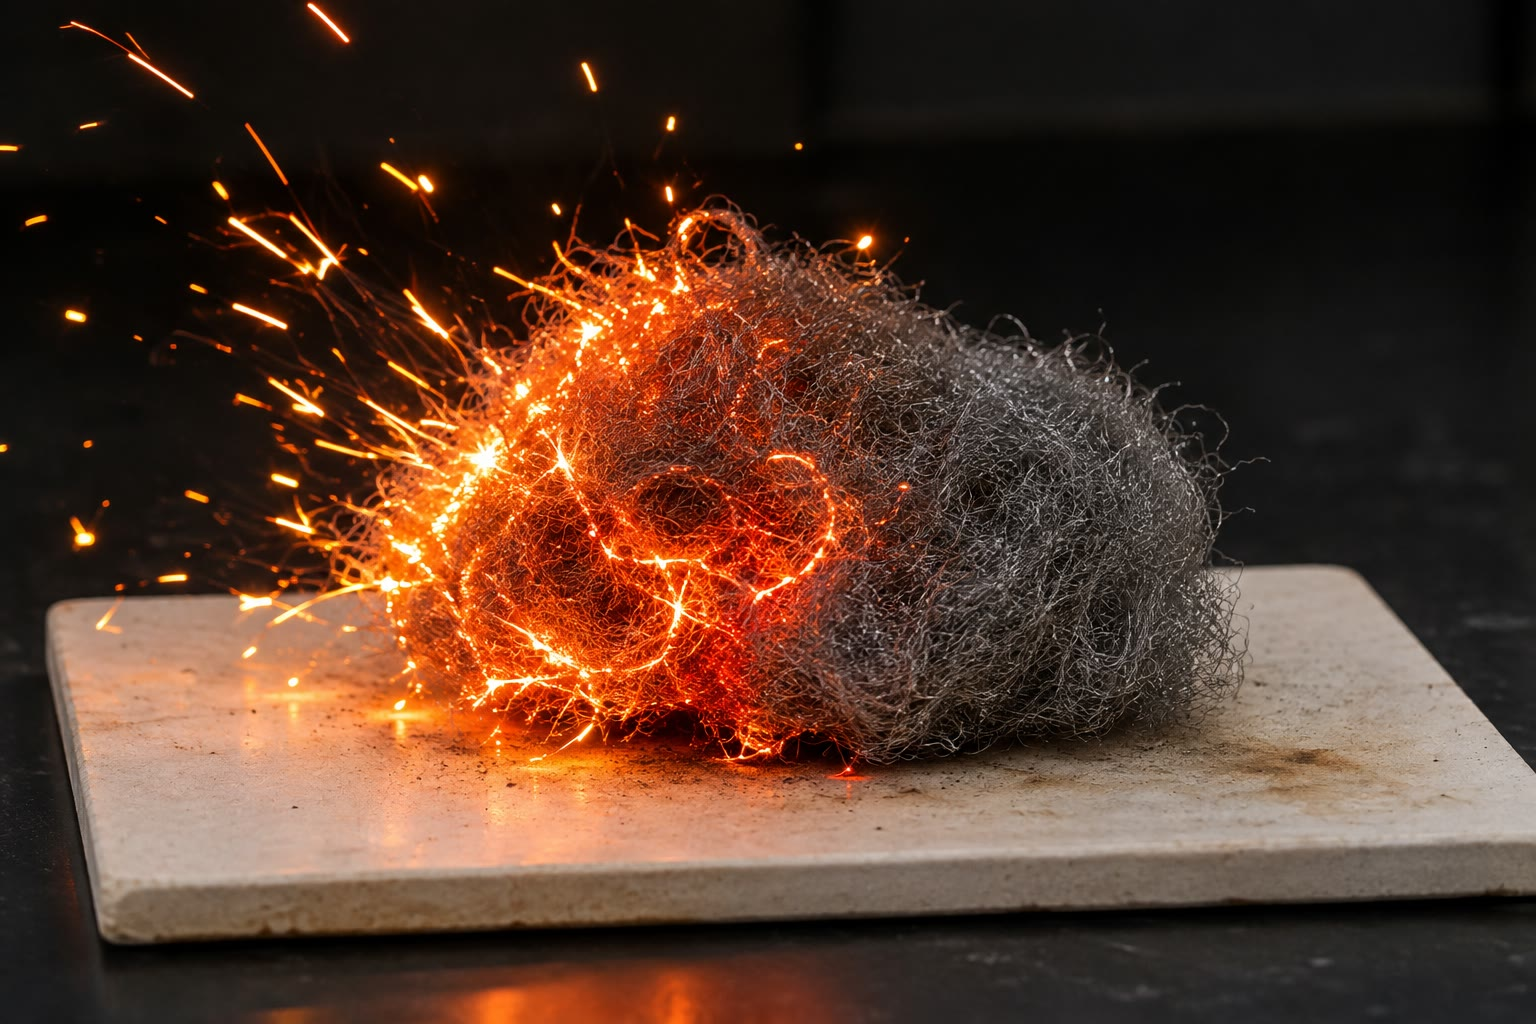
\includegraphics[width=0.5\linewidth]{images/book1/ai/g7-steel-wool-burning.jpg}

{\small Brandende staalwol in het laboratorium: ijzer en zuurstof
reageren.}
\end{omfigure}

\section{Het reactieschema}

\begin{definition}[Reactieschema]\label{def:g7:chemical-reactions:word-equation}
Een \emph{reactieschema}\index{reactieschema} schrijft een \omterm{def:g7:chemical-reactions:reaction}{chemische
reactie} in woorden: links de namen van de \omterm{def:g7:chemical-reactions:reactant}{beginstoffen}, verbonden door
$+$, dan een pijl, en rechts de namen van de \omterm{def:g7:chemical-reactions:reactant}{reactieproducten}. De pijl
lees je als ``reageren tot''.
\end{definition}

\begin{example}[Drie reactieschema's]\label{ex:g7:chemical-reactions:three}
\begin{center}
\begin{tabular}{l}
koolstof $+$ zuurstof $\longrightarrow$ koolstofdioxide\\[2pt]
methaan $+$ zuurstof $\longrightarrow$ koolstofdioxide $+$ water\\[2pt]
ijzer $+$ zuurstof $\longrightarrow$ ijzeroxide
\end{tabular}
\end{center}
\end{example}

\begin{method}[Een reactieschema opschrijven]\label{met:g7:chemical-reactions:write}
\begin{enumerate}
  \item Zoek de \omterm{def:g7:chemical-reactions:reactant}{beginstoffen}: de stoffen die verdwijnen.
  \item Zoek de \omterm{def:g7:chemical-reactions:reactant}{reactieproducten}: de nieuwe stoffen, aangetoond met
        tests.
  \item Schrijf de \omterm{def:g7:chemical-reactions:reactant}{beginstoffen} links en de \omterm{def:g7:chemical-reactions:reactant}{reactieproducten} rechts, met
        een pijl ertussen; nooit een isgelijkteken.
\end{enumerate}
Een stof die aanwezig is maar niet meedoet --- de stikstof van de \omterm{def:g4:air-a-mixture-of-gases:air}{lucht}
rond een vlam --- schrijf je niet op.
\end{method}

\section{Een reactie is een herschikking van atomen}

\begin{proposition}[Atomen worden herschikt]\label{prop:g7:chemical-reactions:rearranged}
Bij een \omterm{def:g7:chemical-reactions:reaction}{chemische reactie} vallen de \omterm{def:g7:atoms-and-molecules:molecule}{moleculen} van de \omterm{def:g7:chemical-reactions:reactant}{beginstoffen} uit
elkaar en verbinden hun \omterm{def:g7:atoms-and-molecules:atom}{atomen} zich op een andere manier tot de
\omterm{def:g7:atoms-and-molecules:molecule}{moleculen} van de \omterm{def:g7:chemical-reactions:reactant}{reactieproducten}. De \omterm{def:g7:atoms-and-molecules:atom}{atomen} zelf worden niet gemaakt en
niet vernietigd: dezelfde \omterm{def:g7:atoms-and-molecules:atom}{atomen}, in dezelfde aantallen, zijn er voor en
na.
\end{proposition}

\begin{example}[Methaan dat verbrandt, molecuul voor molecuul]\label{ex:g7:chemical-reactions:methane}
Als het methaan van een gasfornuis verbrandt, ontmoet één
methaanmolecuul \ce{CH4} twee zuurstofmoleculen \ce{O2}. Hun \omterm{def:g7:atoms-and-molecules:atom}{atomen}
herschikken zich tot één koolstofdioxidemolecuul \ce{CO2} en twee
watermoleculen \ce{H2O}. Voor: 1 koolstof-, 4 waterstof- en 4
zuurstofatomen. Na: 1 koolstof-, 4 waterstof- en $2 + 2 = 4$
zuurstofatomen. Er gaat niets verloren, er komt niets uit het niets.
\end{example}

\begin{omfigure}
\begin{tikzpicture}[font=\small]
  % methane
  \begin{scope}[xshift=0cm]
    \node[aC] (c) at (0,0) {};
    \node[aH] (h1) at (0,0.78) {}; \node[aH] (h2) at (-0.74,-0.3) {};
    \node[aH] (h3) at (0.74,-0.3) {}; \node[aH] (h4) at (0.2,-0.68) {};
    \begin{scope}[on background layer]
      \foreach \h in {h1,h2,h3,h4} \draw[bond] (c.center) -- (\h.center);
    \end{scope}
    \node at (0,-1.2) {1 methaan};
  \end{scope}
  \node at (1.45,0) {$+$};
  % two oxygen molecules
  \foreach \y in {0.45,-0.45} {
    \node[aO] (a) at (2.4,\y) {}; \node[aO] (b) at (3.05,\y) {};
    \begin{scope}[on background layer]
      \draw[bond, line width=1.1pt] ([yshift=1.6pt]a.center) -- ([yshift=1.6pt]b.center);
      \draw[bond, line width=1.1pt] ([yshift=-1.6pt]a.center) -- ([yshift=-1.6pt]b.center);
    \end{scope}
  }
  \node at (2.72,-1.2) {2 zuurstof};
  \draw[->, thick, omProp] (3.8,0) -- (5.0,0);
  % carbon dioxide
  \begin{scope}[xshift=6.3cm]
    \node[aO] (a) at (-0.8,0) {}; \node[aC] (c) at (0,0) {}; \node[aO] (b) at (0.8,0) {};
    \begin{scope}[on background layer]
      \foreach \d in {-1.6,1.6} {
        \draw[bond, line width=1.1pt] ([yshift=\d pt]a.center) -- ([yshift=\d pt]c.center);
        \draw[bond, line width=1.1pt] ([yshift=\d pt]c.center) -- ([yshift=\d pt]b.center);}
    \end{scope}
    \node at (0,-1.2) {1 koolstofdioxide};
  \end{scope}
  \node at (7.8,0) {$+$};
  % two water molecules
  \foreach \x in {8.9,10.6} {
    \node[aO] (o) at (\x,0.2) {};
    \node[aH] (p) at (\x-0.58,-0.25) {}; \node[aH] (q) at (\x+0.58,-0.25) {};
    \begin{scope}[on background layer]
      \draw[bond] (o.center) -- (p.center); \draw[bond] (o.center) -- (q.center);
    \end{scope}
  }
  \node at (9.75,-1.2) {2 water};
  % atom counts
  \node[align=center, font=\footnotesize] at (1.5,-2.0) {voor: 1 C, 4 H, 4 O};
  \node[align=center, font=\footnotesize] at (8.5,-2.0) {na: 1 C, 4 H, 4 O};
\end{tikzpicture}

{\small Methaan dat verbrandt, getekend met molecuulmodellen: de \omterm{def:g7:atoms-and-molecules:atom}{atomen}
van de \omterm{def:g7:chemical-reactions:reactant}{beginstoffen} herschikken zich tot de \omterm{def:g7:chemical-reactions:reactant}{reactieproducten}. Voor en na
tel je dezelfde \omterm{def:g7:atoms-and-molecules:atom}{atomen}.}
\end{omfigure}

\begin{remark}[De moleculen tellen]\label{rem:g7:chemical-reactions:counting}
Het \omterm{def:g7:chemical-reactions:word-equation}{reactieschema} zegt niet hoeveel \omterm{def:g7:atoms-and-molecules:molecule}{moleculen} er reageren: daarvoor
schrijf je de vergelijking op met formules en getallen ervoor. Zulke
vergelijkingen opschrijven, en de juiste getallen vinden, is het
onderwerp van een later hoofdstuk.
\end{remark}

\section{Oefeningen}

\begin{exercise}[$\star$]\label{exo:g7:chemical-reactions:1}
Fysische of \omterm{def:g5:irreversible-changes:chemical-change}{chemische verandering}? IJs dat smelt, een lucifer die
brandt, suiker die \omterm{def:g2:mixing-and-dissolving:dissolve}{oplost}, brood dat geroosterd wordt, een spijker die
roest.
\end{exercise}

\begin{exercise}[$\star$]\label{exo:g7:chemical-reactions:2}
Wat zijn de \omterm{def:g7:chemical-reactions:reactant}{beginstoffen} en de \omterm{def:g7:chemical-reactions:reactant}{reactieproducten} van een \omterm{def:g7:chemical-reactions:reaction}{chemische
reactie}?
\end{exercise}

\begin{exercise}[$\star$]\label{exo:g7:chemical-reactions:3}
Schrijf het \omterm{def:g7:chemical-reactions:word-equation}{reactieschema} op van de \omterm{def:g4:what-a-fire-needs:burning}{verbranding} van koolstof in
zuurstof.
\end{exercise}

\begin{exercise}[$\star$]\label{exo:g7:chemical-reactions:4}
Noem in het \omterm{def:g7:chemical-reactions:word-equation}{reactieschema} ``ijzer $+$ zuurstof $\longrightarrow$
ijzeroxide'' de \omterm{def:g7:chemical-reactions:reactant}{beginstoffen} en het \omterm{def:g7:chemical-reactions:reactant}{reactieproduct}.
\end{exercise}

\begin{exercise}[$\star\star$]\label{exo:g7:chemical-reactions:5}
Als methaan verbrandt, beslaat een koud glas boven de vlam, en het
opgevangen gas maakt kalkwater troebel. Welke \omterm{def:g7:chemical-reactions:reactant}{reactieproducten} tonen
deze twee tests aan?
\end{exercise}

\begin{exercise}[$\star\star$]\label{exo:g7:chemical-reactions:6}
Zink reageert met zoutzuur: het zink verdwijnt, er ontsnappen belletjes
waterstof, en er blijft zinkchloride in de oplossing achter. Schrijf het
\omterm{def:g7:chemical-reactions:word-equation}{reactieschema} op.
\end{exercise}

\begin{exercise}[$\star\star$]\label{exo:g7:chemical-reactions:7}
Kijk naar de figuur met de modellen van methaan dat verbrandt. Tel de
waterstofatomen voor en na de reactie.
\end{exercise}

\begin{exercise}[$\star\star$]\label{exo:g7:chemical-reactions:8}
Waarom is zout \omterm{def:g2:mixing-and-dissolving:dissolve}{oplossen} in water geen \omterm{def:g7:chemical-reactions:reaction}{chemische reactie}, hoewel het zout
uit het zicht verdwijnt?
\end{exercise}

\begin{exercise}[$\star\star$]\label{exo:g7:chemical-reactions:9}
Een houtblok brandt op tot een hoopje as. Leg met het woord
``\omterm{def:g7:chemical-reactions:reactant}{reactieproducten}'' uit waarom de as zoveel lichter is dan het blok.
\end{exercise}

\begin{exercise}[$\star\star$]\label{exo:g7:chemical-reactions:10}
Waterstof verbrandt in zuurstof en geeft alleen water. Schrijf het
\omterm{def:g7:chemical-reactions:word-equation}{reactieschema} op, en zeg met welke test je het \omterm{def:g7:chemical-reactions:reactant}{reactieproduct} kunt
aantonen.
\end{exercise}

\begin{exercise}[$\star\star\star$]\label{exo:g7:chemical-reactions:11}
Twee waterstofmoleculen \ce{H2} reageren met één zuurstofmolecuul \ce{O2}
tot twee watermoleculen \ce{H2O}. Tel de \omterm{def:g7:atoms-and-molecules:atom}{atomen} van elke soort voor en
na, en laat zien dat er geen enkel \omterm{def:g7:atoms-and-molecules:atom}{atoom} gemaakt of vernietigd is.
\end{exercise}

\begin{exercise}[$\star\star\star$]\label{exo:g7:chemical-reactions:12}
Een leerling tekent de \omterm{def:g4:what-a-fire-needs:burning}{verbranding} van koolstof zo: één koolstofatoom
$+$ één zuurstofmolecuul $\longrightarrow$ één koolstofdioxidemolecuul
en één zuurstofatoom dat overblijft. Wat is er mis met deze tekening?
Beschrijf de juiste tekening in woorden.
\end{exercise}

\section{Probleem: In de vlam van een gasfornuis}

\begin{problem}[{Weekendprobleem --- wat er in de vlam van een gasfornuis
verbrandt, wat het oplevert, en hoeveel moleculen meedoen}]
\label{pb:g7:chemical-reactions:1}
Het gas van een keukenfornuis is grotendeels methaan, \ce{CH4}. In zijn
blauwe vlam reageert methaan met de zuurstof van de \omterm{def:g4:air-a-mixture-of-gases:air}{lucht}. In een
laboratorium houdt de docent een koud, droog bekerglas een paar seconden
ondersteboven boven zo'n vlam, keert het dan om, giet er een beetje
kalkwater in en schudt.

\medskip
\noindent\textbf{Deel I --- \omterm{def:g7:chemical-reactions:reactant}{Beginstoffen} en \omterm{def:g7:chemical-reactions:reactant}{reactieproducten}.}
\begin{enumerate}
  \item Noem de twee \omterm{def:g7:chemical-reactions:reactant}{beginstoffen} van deze reactie.
  \item Binnen in het koude bekerglas verschijnen druppeltjes; een
        druppel daarvan kleurt watervrij kopersulfaat blauw. Welk
        \omterm{def:g7:chemical-reactions:reactant}{reactieproduct} toont dat aan?
  \item Het kalkwater wordt troebel. Welk ander \omterm{def:g7:chemical-reactions:reactant}{reactieproduct} toont dat
        aan?
  \item De \omterm{def:g4:air-a-mixture-of-gases:air}{lucht} bevat ook stikstof, dat onveranderd door de vlam gaat.
        Is stikstof een \omterm{def:g7:chemical-reactions:reactant}{beginstof}? Hoort het in het \omterm{def:g7:chemical-reactions:word-equation}{reactieschema}?
\end{enumerate}

\medskip
\noindent\textbf{Deel II --- Het \omterm{def:g7:chemical-reactions:word-equation}{reactieschema}.}
\begin{enumerate}[resume]
  \item Schrijf het \omterm{def:g7:chemical-reactions:word-equation}{reactieschema} van de reactie op.
  \item Is de \omterm{def:g4:what-a-fire-needs:burning}{verbranding} van methaan een fysische of een \omterm{def:g5:irreversible-changes:chemical-change}{chemische
        verandering}? Geef twee redenen.
  \item Schrijf de formules op van de vier stoffen van de reactie.
\end{enumerate}

\medskip
\noindent\textbf{Deel III --- \omterm{def:g7:atoms-and-molecules:molecule}{Moleculen} tellen.}
Elk methaanmolecuul dat verbrandt, reageert met twee zuurstofmoleculen
en levert één koolstofdioxidemolecuul en twee watermoleculen.
\begin{enumerate}[resume]
  \item Tel de koolstof-, waterstof- en zuurstofatomen in één
        methaanmolecuul en twee zuurstofmoleculen samen.
  \item Tel ze in één koolstofdioxidemolecuul en twee watermoleculen
        samen. Wat valt je op?
  \item De vlam verbrandt 10 methaanmoleculen. Hoeveel zuurstofmoleculen
        gebruikt ze?
  \item Hoeveel koolstofdioxidemoleculen maakt ze?
  \item Hoeveel watermoleculen maakt ze?
\end{enumerate}
\end{problem}
